\section{Durchführung}
\label{sec:Durchführung}

Die verwendete Messaperatur ist in Abbildung \ref{fig:Aufbau} skizziert. 

\begin{figure}
  \centering
  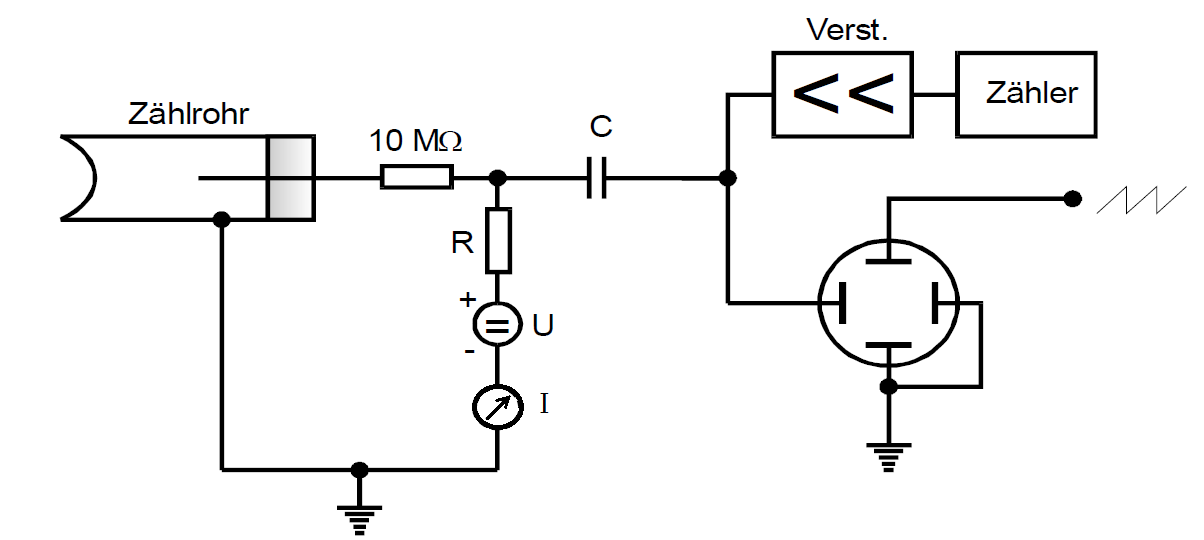
\includegraphics[scale=0.3]{content/Aufbau.png}
  \caption{Skizze der Messaperatur [1]}
  \label{fig:Aufbau}
\end{figure}

Die durch ein einfallendes Teilchen verursachte Ladung $Q$ fließt über den Widerstand $R$
ab und erzeugt somit einen Spannungsimpuls. Dieser wird über einen Kondensator 
ausgekoppelt und mit einem Zähler gezählt bzw. mit Hilfe eines Oszilloskopes sichtbar
gemacht. \\
Der Versuch kann in drei Versuchsteile gegliedert werden. \\

Im ersten Teil wird die Charakteristik des Geiger-Müller-Zählrohrs untersucht. Dabei 
wird die Impulsrate bei etwa $\SI{100}{\per\second}$ gehalten, um den Einfluss der 
Totzeit möglichst gering zu halten. Desweiteren wird eine Messdauer von $\SI{100}{\second}$
gewählt, damit der Fehler unter $\SI{1}{\percent}$ liegt. Dann wird die Zählrohrspannung
in $\SI{20}{\volt}$ von $\SI{300}{\volt}$ auf $\SI{700}{\volt}$ erhöht und die 
registrierten Impuls $N$ sowie die Stromstärke $I$ gemessen. \\

Im nächsten Versuchsteil werden Messungen mit Hilfe des Oszilloskopes durchgeführt. 
Zunächst wird bei einer Spannung von $U = \SI{350}{\volt}$ die Strahlintensität so 
eingestellt, dass nur der Primärimpuls auf dem Bildschirm zu sehen ist. Bei 
gleichbleibender Strahlintensität wird daraufhin die Spannung auf $\SI{700}{\volt}$
erhöht und die qualitative Veränderung beobachtet. Dabei wird der Abstand zwischen
dem Primärimpuls und den auftretenden Nachentladungen ermittelt. Außerdem wird bei 
beiden Spannungen $T_\text{T}$ am Oszilloskop ald Breite des Primärimpulses 
abgelesen. Mit Hilfe des Oszilloskopes wird auch versucht die Erholungszeit $T_\text{E}$
abzuschätzen. \\

Mit der angesprochenen Zwei-Quellen-Methode wird im letzten Versuchsteil die Totzeit
des Zählrohrs bestimmt. Hierzu wird die Zählrohrspannung auf eine Spannung geregelt, 
welche sich nach den vorherigen Messungen als geeignet herausstellt ($\SI{500}{\volt}$).
Nun folt das Verfahren der Zwei-Quellen-Methode: Zunächst wird die Zählrate der ersten
Spannungsquelle gemessen. Dann wird die zweite Quelle hinzugefügt und eine weitere 
Messung durchgeführt. Anschließend wird die erste Quelle entfernt und nur noch die 
Zählrate der zweiten Quelle gemessen. Der Messzeitraum beträgt dabei immer $\SI{100}{\second}$.
Es wird bei den Messungen darauf geachtet, dass die Quellen nicht verschoben 
werden und die Zählrate von beiden Quellen gleichzeitig geringer ist als die Summe 
der Zählraten der einzelnen Quellen. \\